\chapter{Autopolarización de Base}
\section{Análisis teórico}
La segunda sección de este trabajo práctico consistirá en el análisis de la autopolarización de 
base para un transistor bipolar de un juntura. Primeramente se estudiará la base del funcionamiento
en dicha configuración para luego aplicarlo a diversos modelos de transistores provistos 
por la cátedra. \par 
El circuito inicial propuesto es el siguiente:

\begin{figure}[H]
    \centering
    \begin{center}
        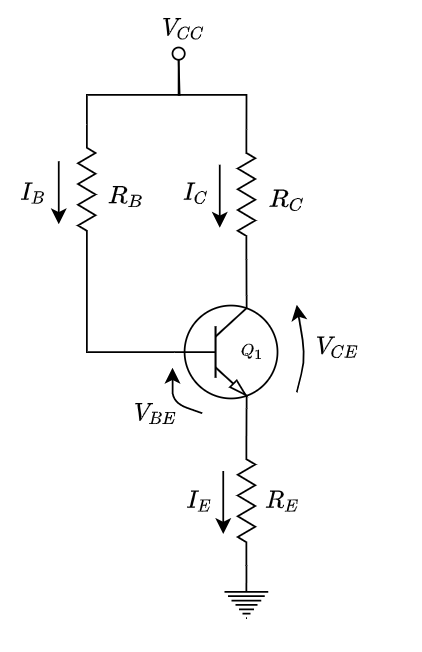
\includegraphics[width=0.3\textwidth]{polarizacion_de_base/Imagenes/circuito_polarizacion_base.png}
        \label{circuito_ejercicio_2}
    \end{center}
    \vspace{-8mm}
    \caption{Circuito para Autopolarización de base}
\end{figure}
Considerando que tanto la base como el colector comparten un node común, el mismo se puede 
separar como si fueran dos fuentes diferentes, una vez realizado este proceso se aplica 
el teorema de Thevenin obteniéndose el equivalente:
\begin{equation}
    V_{th}= V_{cc} \hspace{20mm} R_{th}=R_B 
    \label{eq_thevenin} 
\end{equation}
Aplicando las ecuaciones despejadas de [\ref{eq_thevenin}] en el circuito propuesto [\ref{circuito_ejercicio_2}]
se simplifica el circuito a la expresión:

\begin{figure}[H]
    \centering
    \begin{center}
        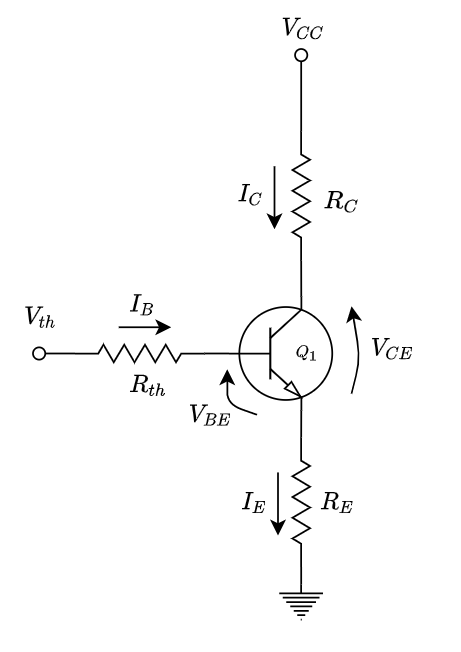
\includegraphics[width=0.3\textwidth]{polarizacion_de_base/Imagenes/circuito_polarizacion_base_thevenin.png}
        \label{circuito_ejercicio_2_thevenin}
    \end{center}
    \caption{Circuito para Autopolarización de base con Thevenin}
\end{figure}
Por otro lado, para este caso en particular se puede apreciar la presencia de la 
resistencia en el emisor ()$R_E$), lo que nos permite protegernos de las grandes fluctuaciones 
que puede tener la ganancia de corriente en un BJT ($h_{fe}$). De esta manera, se pueden 
despejar los parámetros de la malla de salida en función de los parámetros de la malla 
de entrada. Obteniéndose las siguientes expresiones: \par 
\begin{equation}
    \vspace{8mm}
    I_C=\frac{V_{th}-V_{BE}}{R_E\left(\frac{1+h_{fe}}{h_{fe}}\right)+\frac{R_{th}}{h_{fe}}}
    \label{eq_I_c}
\end{equation}

\begin{equation}
    V_{CE}=V_{CC}-I_C(R_C+R_E)
    \label{eq_V_CE}
\vspace{8mm}
\end{equation}

\section{Selección de componentes}

Contando entonces con el transistor bipolar BC547, se buscan los valores para $R_C$, $R_B$ y $R_E$ tal que se cumplan las condiciones de diseño.
En este caso se desea $I_c =  2mA$. Es necesario buscar en la hoja de datos del transistor los datos de la tabla \ref{table:parametros transistor}.
\begin{table}[ht]
    \centering
    \begin{tabular}{l|l|l|l}
                  & Min  & Típica & Máximo \\ \hline
    $\beta$       & 100  &        & 800    \\ \hline
    $V_{BEon}$    & 0.58 & 0.66   & 0.7    \\ \hline
    $V_{CEsat}$   &      & 0.09   & 0.25  
    \end{tabular} 
    \caption{}\label{table:parametros transistor}
\end{table}

Como condición de correcto funcionamiento se tiene la relación $V_{CE} < V_{CEsat}$ se aplica sobre la ecuación \ref{eq_V_CE}.
\begin{equation}
    V_{CEsat}<V_{CC}-I_C(R_C+R_E)
    \label{eq_V_CEsat}
\end{equation}
Lo cual se puede despejar para obtener una relación directa entre las resistencias de base y de emisor.
\begin{equation}
    \frac{V_{cc} -V_{CEsat}}{I_c} > R_C + R_E
    \label{eq_cota_sup_RC_RE}
\end{equation}
Ahora aplicando el peor caso posible para $V_{CEsat}$ de la tabla \ref{table:parametros transistor} y teniendo en cuenta el valor deseado para $I_c$ se arriba a la cota superior para la suma entre las resistencias.
\begin{equation}
    4375< R_E + R_C
    \label{cota_numerica}
\end{equation}
Debido a la disponibilidad de elementos en este caso se selecciona $R_E = R_C = 1.5k\Omega$.
Ya que se trata de valores de $h_{fe}$ altos la aproximación $\frac{1+h_{fe}}{h_{fe}}\approx 1$ es correcta. Por lo tanto con los valores propuestos para $R_E$, la aproximación mencionada y la ecuación \ref{eq_I_c} se puede proponer lo siguiente.
\begin{equation}
    \frac{V_{th} - V_{BEon}}{I_c} - R_E = \frac{R_B}{\beta}
    \label{eq_relacion_R_B}
\end{equation}
Para este caso en especifico $h_{fe}$ presenta una gran variación, por lo tanto hay un rango de valores posibles para $R_B$. Teniendo en cuenta los casos limitesy las condiciones de diseño impuestas se presentan las siguientes cotas.
\begin{equation}
    2350 h_{fe min} < R_B < 2350 h_{fe max}
\end{equation}
\begin{equation}
    258.5k\Omega < R_B < 1.88M\Omega
\end{equation}
Asumiendo un valor de $\beta \approx 330$, bajo el fundamento de que el transistor a usar es de la serie B, se decide sobre una $R_B = 780k\Omega$.
Entonces los valores a utilizar son
\begin{center}
    $R_E = 1500\Omega$  $R_C = 1500\Omega$ $R_B = 780 k\Omega$
\end{center}

A partir de estos nuevos parámetros, empleando la \ref{eq_I_c} y \ref{eq_V_CE} se encuentra el punto de polarización.
\begin{equation}
    I_{CQ} = 1.99mA   \hspace{5mm} V_{CEQ} = 3.01V
    \label{eq_Punto_Q_teorico}
\end{equation}

\section{Casos de aplicación}

Se busca en esta sección medir y contrastar 
el punto de polarización experimental y el calculado en la ecuación 
\ref{eq_Punto_Q_teorico}.
Luego de armar el circuito propuesto 
en la figura \ref{circuito_ejercicio_2}, se mide la caída de tensión en $R_C$ a fin de obtener $I_{CQ}$. A su vez se mide $V_{CEQ}$. El circuito a medir se encuentra en la figura \ref{fig_circuito_fisico}.

\begin{figure}[H]
    \centering
    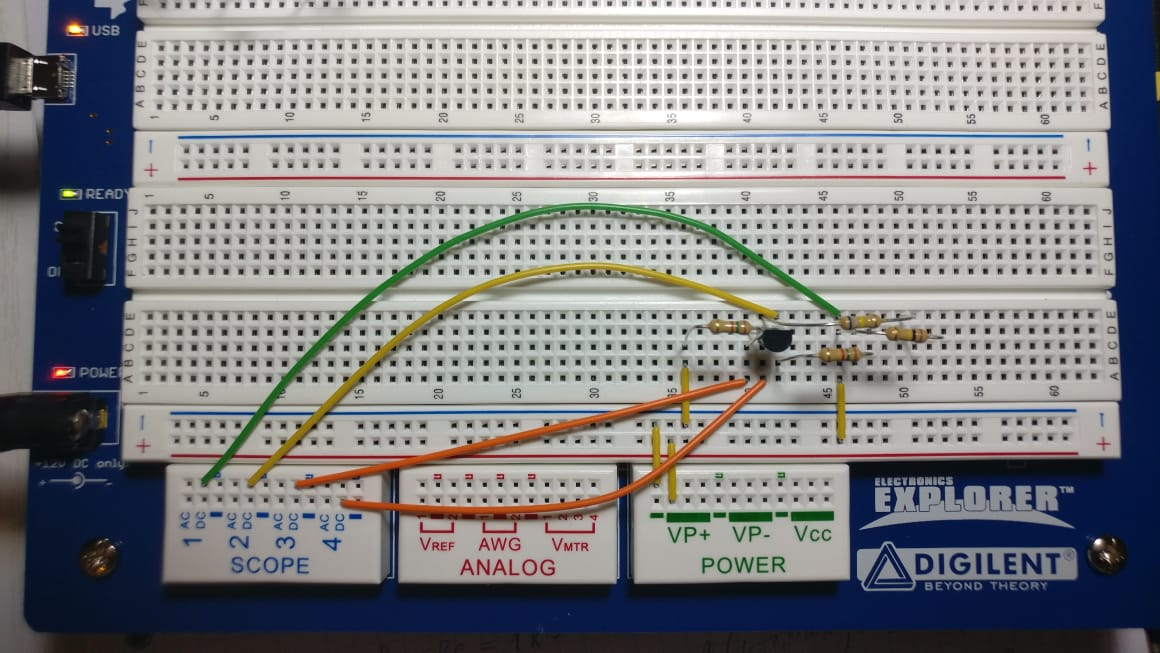
\includegraphics[scale = 0.3]{polarizacion_de_base/Imagenes/circuito_polarizado.jpeg}
    \caption{Implementación del circuito}\label{fig_circuito_fisico}
\end{figure} 


Conociendo $I_{CQ}$ experimentalmente, y los valores nominales de $R_E$ y $R_B$ con la ecuación \ref{eq_I_c} se puede despejar $\beta$ para esta configuración. También se corrobora esta cuenta calculando la corriente de base y dividiendo la corriente de colector por ella.
Ambos procedimientos resultan en valores muy similares
Los resultados se detallan en la tabla \ref{tabla_resultados_polarizacion}.

\begin{table}[ht]
    \centering
    \begin{tabular}{|l|l|l|l|l|}
    \hline
          & $I_{CQ}$  & $V_{CEQ}$ & $V_{BEQ}$ & $\beta$ \\ \hline
    $Q_1$ & $1,76 mA$ & $3.65 V$ & $0.66 mV$  & $236$   \\ \hline
    $Q_2$ & $1.93 mA$ & $3.21 V$  & $0.66 mV$ & $278$   \\ \hline
    \end{tabular}
    \caption{}\label{tabla_resultados_polarizacion}
\end{table}
Para contrastar la dispersión de valores entre transistores, se lleva a cabo la misma experiencia con otro transistor del mismo modelo.
Los resultados están dentro de lo esperado. En primer lugar la $V_{BEQ}$ se encuentra exactamente en el lugar marcado como típico por el fabricante para ambos casos.
Respecto a la $I_{CQ}$ el transistor que cuenta con la $\beta$ mas parecida a la asumida en el diseño, presenta un valor experimental muy cercano al deseado. Mientras que para $Q_1$ está dentro de las posibilidades aceptables es mas lejano. 
Al contar con la serie B del BC547, $\beta$ se encuentra correctamente dentro de las cotas previstas por el fabricante.

